\documentclass[10pt,a4paper]{article}
\usepackage[T1]{fontenc}
\usepackage[utf8]{inputenc}
\usepackage{lmodern}
\usepackage{enumerate}
\usepackage{fancyhdr}
\usepackage{lastpage}
\usepackage{graphicx}
\pagestyle{fancy}
\usepackage[clock]{ifsym}
\usepackage{fancyhdr}
\usepackage{hyperref}

\author{Stanisław Deja}
\title{Neural Networks in Autonomous Vehicles \\
\small Based on "Driving Darwin" program}
\date{\today}
\begin{document}

\lhead{Stanisław Deja}
\rhead{Neural Networks in Autonomous Vehicles}
\maketitle

\tableofcontents
\section{Neural Network}
At its core, a neural network is a computational model inspired by the way biological neural networks in the human brain work. It's used in machine learning to recognize patterns and make intelligent decisions. Let's break down the key components of a neural network.
\subsection{Neurons(Nodes)}
    \begin{itemize}
        \item In a neural network, you have nodes, also called neurons. These nodes are organized into layers: an input layer, one or more hidden layers, and an output layer.
        \item Each neuron in a layer is associated with a numerical value called an activation.
    \end{itemize}
\subsection{Weights}
    \begin{itemize}
\item Each connection between neurons has a weight associated with it. These weights determine the strength of the connection between neurons.
\item Mathematically, if we denote the input to a neuron as $x$ and and the weight as $w$, the weighted input is $w*x$.
    \end{itemize}
\subsection{Activation Function}
\begin{itemize}
    \item After calculating the weighted sum, an activation function is applied to introduce non-linearity into the system. This allows neural networks to learn complex patterns.
    \item Common activation functions include the sigmoid function \begin{math}\sigma(x)=\frac{1}{(1+e^-x)}\end{math}
\end{itemize}
\subsection{Feedforward Process}
\begin{itemize}
\item The information flows through the network in a process called feedforward. Each layer's neurons receive input from the previous layer, apply the weights, sum them up, and pass the result through the activation function
\item Mathematically, for a neuron in layer i, the output $y_{i}$ is is calculated as: $y_{i}=\Sigma_{j} weights_{ij}*input_{j}$

\end{itemize}
\section{Cars Brain - What if we give Neural Network to a car?}
\subsection{First we need to consider following things}
\begin{itemize}
    \item \textbf{Input to the Artificial Brain:} What information should be fed into the system to facilitate learning and decision-making?
    \item \textbf{Handling the Outcome:} Once the artificial brain processes the input, how should the outcomes be utilized or acted upon?
\end{itemize}
\subsection{Input for the cars brain}
Cars navigate roads smoothly without hitting edges.
Focus on car-to-road-edge distance.
Check distance in various directions.
Input them as an array to our Neural Network.
\begin{figure}[!h]
	\centering
    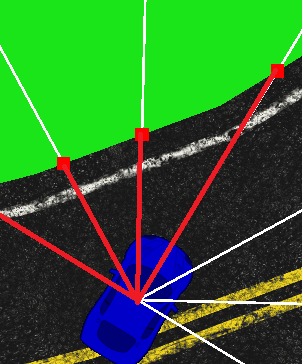
\includegraphics[scale=0.5]{cardist.png}
	\centering
    \caption{\tiny Distance to the edge of the road in directions(Red lines)}
\end{figure}
\subsection{Output of the Network}
As the brain of our car "knows" about its surroundings
Maybe its good idea to let it steer the car
Let the output of the network be the direction of movement and velocity 
\subsection{Testing the idea}
Let's finally give it a brain a plug everything in
Put it on the road and...
It bumps into to the edge of the road. \textbf{Why?}
Its brain is very primitive \textbf{It needs to learn and evolve} 
\begin{figure}[!h]
	\centering
    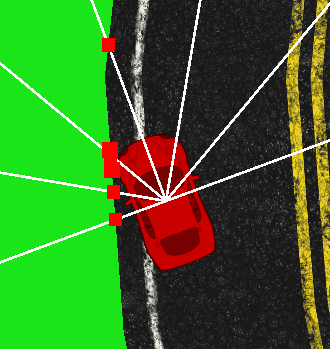
\includegraphics[scale=0.5]{cardump.png}
	\centering
    \caption{\tiny Car is not clever for now}
\end{figure}
\subsection{Evolution}
\begin{figure}[!h]
	\centering
    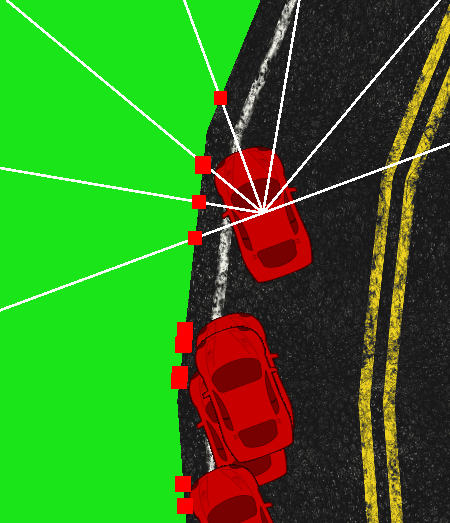
\includegraphics[scale=0.5]{evolution.png}
	\centering
    \caption{\tiny One of the cars is better}
\end{figure}
\begin{enumerate}
    \item Let’s take a bunch of cars and give each one an unique random brain.
    \item Well they still bump into the edge of the road
    \item \textbf{However} One of them managed to travel Further than others. That means its brain was the \textbf{smartest}
    \item Let’s create a new generation of cars. \textbf{However} this time we will give each new car slightly modified version of
    the best brain from the previous generation
    \item In that way the new generation will ”learn” from the previous one
\end{enumerate}
\Large{Repeatition}
\normalsize
\begin{itemize}
    \item We can repeat process described above over and over again
    \item That way each new generation will learn from its predecessors
    \item and stack its knowledge, until...
    \item eventually, we will get a car that is able to drive on its own
\end{itemize}

\section{Progress over Generation}
    In Figure 4 we can see data gathered from "DrivingDarwin" program representing distance the best car from given generation has traveled. Each generation makes significant progress.
    Until generation 7 is able to fully drive on the road
\begin{figure}[!h]
    \centering
    \begin{tabular}{||c || c||}
        Generation & Distance \\
        \hline
        1  & 12\\
        \hline
        2  & 34\\
        \hline
        3  & 52\\
        \hline
        4  & 54\\
        \hline
        5 & 61\\
        \hline
        6 & 91\\
        \hline
        7 & inf\\
    \end{tabular}
\caption{\tiny{Data collected on 21.12.2023 using ”DrivingDarwin” program}} 
\end{figure}

\section{Further Reading}
\Large{Sources}\\
    \begin{tabular}{||c||c}
       \textbf{\footnotesize{Project page* }}&\footnotesize{ \url{https://github.com/stachurski2k/DrivingDarwin}}
    \end{tabular}\\
    \break \break \break
\Large{Links}\\
    \begin{tabular}{||c||c}
\textbf{\scriptsize{Inspiration}} & \scriptsize{ \url{https://youtu.be/hfMk-kjRv4c?si=KWKiRY9hVDP_R-bV}}\\
\hline
\textbf{\scriptsize{Neural Networks}} & \scriptsize{ \url{https://youtu.be/aircAruvnKk?si=-pxO5wa7qVt-1eHh}}\\
\hline
\textbf{\scriptsize{Road Generation}}& \scriptsize{ \url{https://youtu.be/RF04Fi9OCPc?si=GgaL0ujYB1aqEibW}}\\
    \end{tabular}\\
    \break \break \break
\footnotesize{
* ”Driving Darwin” was fully developed by the author of this presentation, it covers
much more advanced concepts than presented such as implementation of Neural
Network from scratch and generator of bezier curves. Their description can be found
in the documentation of the project.}
\end{document}
